\documentclass{article}

% packages
\usepackage{array}
\usepackage{graphicx}
\usepackage{lastpage}
\usepackage{fancyhdr}
\usepackage{color}
\usepackage{float}
\usepackage[hidelinks]{hyperref}

% page margins
\addtolength{\topmargin}{-0.75in}
\addtolength{\oddsidemargin}{-1.0in}
\addtolength{\evensidemargin}{-1.0in}
\addtolength{\textwidth}{2.0in}
\addtolength{\textheight}{1.5in}

% header and footer
\pagestyle{fancy}
\fancyhf{}
\lhead{Fault-Tolerant Quadcopter}
\rhead{\textit{Vaughn, Mayank, Cooper}}
\cfoot{\thepage\ of \pageref{LastPage}}
\rfoot{\today}

% custom commands
\newcommand{\HREF}[2]{{\color{blue}\underline{\smash{\href{#1}{#2}}}}}
\newcommand{\HREFA}[2]{\textcolor{blue}{\underline{\smash{\href{#1}{#2}}}}}

% metadata
\title{ECE 453 Project Proposal}
\author{Vaughn Kottler}
\author{Mayank Katwal}
\author{Cooper Green}

\begin{document}

\begin{center}
	{\Huge Fault-Tolerant Quadcopter}
    \break

	{\large\textbf{ECE 453 Project Proposal} (Fall 2018)}

	{\large University of Wisconsin-Madison}
    \break

	{\large\textit{Vaughn Kottler, Mayank Katwal, Cooper Green}}
\end{center}

\section{Abstract}

This document serves as the formal, semester-project proposal to be vetted by
the course instructor:
\HREF{https://directory.engr.wisc.edu/ece/Faculty/Krachey_Joe/}{Joe Krachey}.
We have additional
\HREF{https://fault-tolerant-quadcopter.readthedocs.io/en/latest/}
{online documentation} that we plan to keep in sync with our project's scope
and current progress.

\section{Executive Summary}

\subsection{Problem Statement}

Seemingly no ``multi-vehicle fleet'' or autonomous-flight capable drone
technology is available to interact with in the consumer market. Similarly,
open-source hardware and software in the ``DIY drone'' ecosystem cannot be
easily converted or augmented to solve that problem.

We identified this problem while exploring learning objectives related to
developing skills for working in aerospace avionics and software. We believe
that gaining relevant experience with this problem space requires
designing, testing and building a custom flying machine.

\subsection{Proposal}

We intend to build a \textbf{quadcopter} plus
\textbf{ground station} and \textbf{web-based user interface}.
We have chosen to call this project the
\textbf{fault-tolerant quadcopter}. This name reveals one of our
design goals that will be covered in a future section. 

With respect to the problem statement (and single-semester timeline), we do
not anticipate delivering a polished technical solution to any of the specific
deficiencies we identify in the ``free and open-source'' ecosystem. We have
tentatively planned to continue working on this project until our source
repository \HREF{https://github.com/vkottler/senior-design}{on GitHub}
represents completed work to a well-defined scope that may differ from
this course project's scope.

\pagebreak

\subsection{Concept of Operation}

The essence of what we would like to create is best captured by 
\textbf{Figure \ref{fig:conops}}.

\begin{figure}[H]
	\centering
	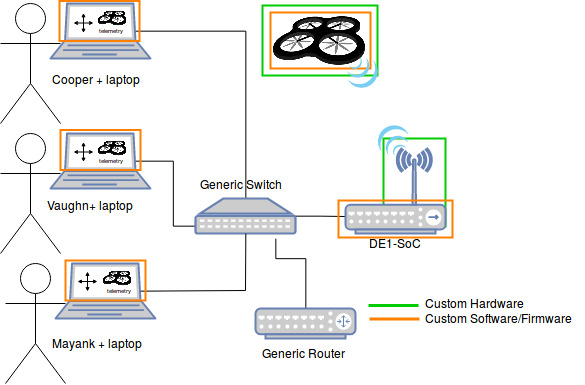
\includegraphics[width=4in]{../src/im/conops}
	\caption{The intended physical configuration.}
	\label{fig:conops}
\end{figure}

Our presentation content goes into more detail about how this architecture
fundamentally differs from what is available in the consumer market. We
believe the strength of this topology is fully realized during final
integration stages and the development of actual control algorithms for flight.
A graphical interface displaying diagnostic information is essential to
vehicle development of any kind and exposing this interface directly to our
workstations opens up opportunities for extremely tight development loops
(imagine if you could change configurations or even upload new code mid-flight
via this interface). We emphasize that the user interface is not just a
convenient or heavily styled view of data but a tool we will use throughout
the lifecycle of this project.

\subsection{Overview}

This project is designed for three major bodies of work that were
mentioned above but are better captured by \textbf{Figure \ref{fig:high-level}}:

\begin{figure}[H]
	\centering
	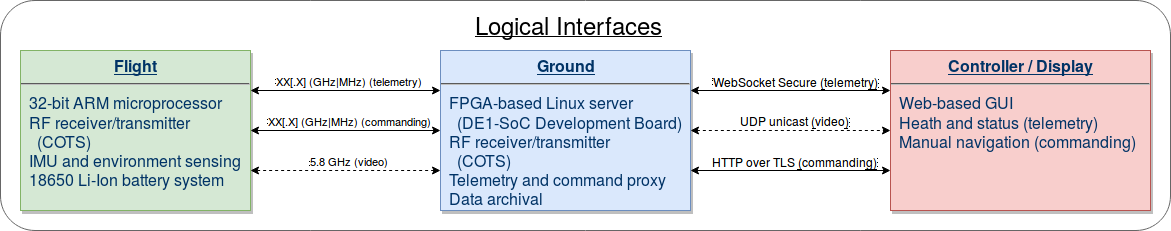
\includegraphics[width=\linewidth]{../src/im/top_level}
	\caption{High-level overview of the major components and
		their interfaces.}
	\label{fig:high-level}
\end{figure}

\noindent This high-level architecture is inspired by existing aerospace
avionics and software systems that we have done research on
and have some first-hand experience with.

\section{Technical Features and Goals}

Note that we focus on system-level goals over specific technical requirements
of individual pieces. Our limited experience in this problem space
makes an attempt at the latter not valuable (i.e. battery life, thrust and
payload capability, etc.).

\subsection{Telemetry Viewing}

Initially, a list of channel names and corresponding values (with staleness)
in a table format. This can grow in complexity to incorporate more interesting
visualizations, potentially incorporating an annotated model of the vehicle
itself.

\subsection{Manual Commanding}

A set of user inputs that can dispatch requests to the vehicle, with feedback
indicating the result of the request (accepted, rejected, couldn't send, etc.).

\subsection{Holding-Pattern Stability}

Support a flight algorithm that enables high-fidelity control over
motion of the vehicle.

\subsection{Fault Tolerance}

A vehicle that is \textit{single-fault tolerant} is capable of continuing
nominal operation after experiencing any arbitrary failure in a well-defined
\textit{fault space}. We aim to implement single-fault tolerance by:

\begin{enumerate}
	\item Limiting the initial fault space to a ``loss of ground station
		heartbeat'' event
	\item Executing a ``landing maneuver'' upon fault detection
	\item Iteratively hardening our design to a broader fault space,
		time permitting
\end{enumerate}

\section{Milestones}

\noindent We recognize some intermediate milestones that will need to be reached
before an \textit{automatic flight-termination system} described above can be
expected to function. Note that we expect to parallelize completion of these
milestones when possible.

\subsection{Establish wireless communication between the vehicle and ground station}

Estimated hours of work: \textbf{40}
\vspace{0.25cm}

\noindent
Involves custom firmware/software for the DE1-SoC and an ARM microcontroller
development board. This comes with the initial burden of establishing a
build system and efficient workflow for development on these two platforms.

\subsection{Establish percentage-based throttle control over each motor}

Estimated hours of work: \textbf{8}
\vspace{0.25cm}

\noindent
Requires interfacing with an ESC (electronic speed controller) via PWM signal.
this won't take as long as other firmware tasks because a base is established
at this point. This control will be done from a command-line interface on
the DE1-SoC, which will require implementing an ``application layer protocol''
on top of the wire-level protocol used by the radios.

\subsection{Establish manual-commanding capability from a web-based user interface}

Estimated hours of work: \textbf{25}
\vspace{0.25cm}

\noindent
Requires completing the initial user interface as well as the server-side
software capable of dispatching hardware tasks to the previously completed
lower layers.

\subsection{View live telemetry from a web-based user interface}

Estimated hours of work: \textbf{15}
\vspace{0.25cm}

\noindent
This involves defining a data structure for telemetry packets that will
be easily serializable for our wire-level protocol mediums and composable
visual elements to display data.

\subsection{Sense angular velocity via gyroscope and force experienced via IMU}

Estimated hours of work: \textbf{20}
\vspace{0.25cm}

\noindent
Previous experience interfacing with gyroscopes and intertial-measurement
units allows us to proceed intelligently with respect to these data paths.
Choosing the right sensors and architecting firmware to allow the full data
rate (some digital filtering applied) to propagate into a control algorithm
is the essence of the task.

\subsection{Develop a control algorithm to fly in a stable hover or holding pattern}

Estimated hours of work: \textbf{8}
\vspace{0.25cm}

\noindent
With the data pipeline implemented all the way through to the user interface,
this should only require implementing and tuning PID control loops that
drive PWM signals to the ESC based on gyroscopic and inertial inputs.
The user interface is a key component that allows this development task
to be expedited.

\subsection{Extend control algorithm to control for velocity in three axes}

Estimated hours of work: \textbf{4}
\vspace{0.25cm}

\noindent
This should only require injecting new ``setpoints'' into the functional
control algorithm developed previously. It is not known at this time whether
or not it will be possible to use setpoints associated with actual units of
velocity, it may end up boolean or throttle-based.

\subsection{Sense relative altitude}

Estimated hours of work: \textbf{10}
\vspace{0.25cm}

\noindent
An altimeter or other sensing technology has not been chosen, we can't
accurately characterize the difficulty of this task yet.

\subsection{Extend control algorithm to control for a specific \textit{delta-z} }

Estimated hours of work: \textbf{2}
\vspace{0.25cm}

\noindent
If altitude can be measured to some degree of accuracy, injecting a new
setpoint into the control algorithm was demonstrated previously which should
make this straightforward.

\section{Roles and Responsibilities}

\begin{quote}
	\textit{``A problem well stated is a problem half
	solved.'' - Charles Kettering}
\end{quote}

\noindent Distribution of work and responsibilities has been discussed and the
following summaries represent a consensus reached on initial roles and task
delegation.

\subsection{Vaughn Kottler}

\begin{description}
	\item [Flight Hardware] Final design and assembly of the quadcopter.
		Validation of component selection to ensure flight is feasible.
	\item [Flight Software] The firmware image flashed to the flight
		computer. Includes necessary control algorithms and runtime
		configurability.
	\item [Project Oversight] Track project progress and maintain
		documentation.
\end{description}

\subsection{Mayank Katwal}

\begin{description}
	\item [Telemetry Display] A web-based dashboard that summarizes the health
		and status of the quadcopter during flight.
	\item [Vehicle Control Interface] A web-based user interface that allows
		manual control of the quadcopter during flight.
	\item [Data and Command APIs] User programs that expose flight data
		and command capability to client browsers via HTTP over TLS requests.
\end{description}

\subsection{Cooper Green}

\begin{description}
	\item [Ground Station] Hardware asbstraction layer source code and
		mezzanine board implementation. A coherent and well-defined interface
		to the hardware from user programs.
	\item [Radio Frequency Communication] Choice of frequency bands and
		protocols used to send and receive data with radio modules.
	\item [Telemetry Storage] A data archival system for post-flight analysis.
\end{description}

\section{Detailed Block Diagrams}

\subsection{Quadcopter}

For the flight vehicle, we intend to pursue an implmentation depicted in
\textbf{Figure \ref{fig:quadcopter}}:

\begin{figure}[H]
	\centering
	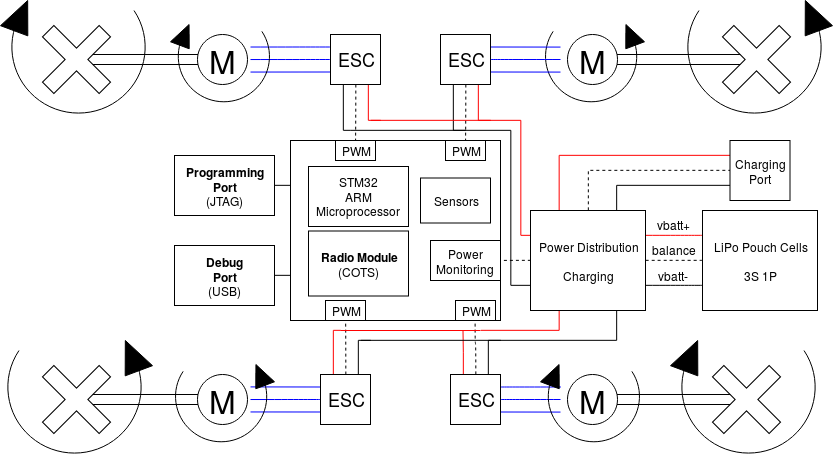
\includegraphics[width=\linewidth]{../src/im/quadcopter}
	\caption{Block diagram view of the quadcopter.}
	\label{fig:quadcopter}
\end{figure}

\noindent{\Large Responsible Engineer: \textbf{Vaughn}}

\pagebreak

\subsection{Ground Station}

For the ground station, we intend to pursue an implmentation depicted in
\textbf{Figure \ref{fig:ground_station}}:

\begin{figure}[H]
	\centering
	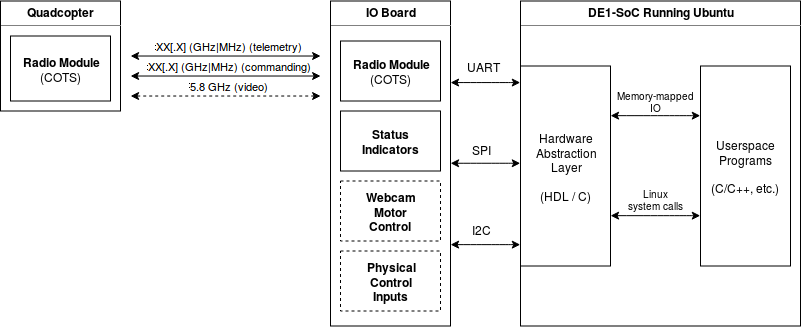
\includegraphics[width=\linewidth]{../src/im/ground_station}
	\caption{Block diagram view of the ground station.}
	\label{fig:ground_station}
\end{figure}

\noindent{\Large Responsible Engineer: \textbf{Cooper}}

\pagebreak

\subsection{Display and Controller}

For the display and control interface, we intend to pursue an
implmentation depicted in \textbf{Figure \ref{fig:display_controller}}:

\begin{figure}[H]
	\centering
	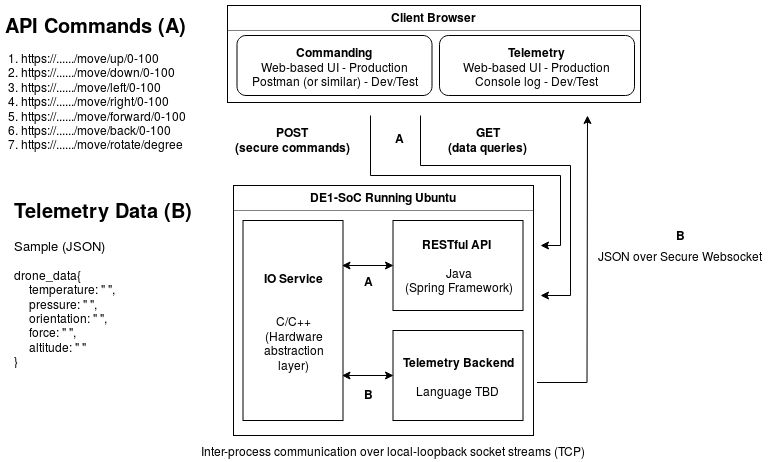
\includegraphics[width=\linewidth]{../src/im/display_controller}
	\caption{Block diagram view of the display and control user
		interface.}
	\label{fig:display_controller}
\end{figure}

\noindent{\Large Responsible Engineer: \textbf{Mayank}}

\pagebreak

\section{Cost Estimation}

This is our estimate of what items are required to complete this
project. Items listed as having zero cost were provided to us or are things
that we already previously owned.

\begin{center}
{\renewcommand{\arraystretch}{1.5}
\begin{tabular}{|p{2in}|p{3in}|p{0.6in}|p{0.65in}|}
    \hline
    \multicolumn{4}{|c|}{\textbf{Quadcopter}} \\
    \hline
    Item (as hyperlink) & Purpose & Quantity & Total Cost \\
    \hline
    \HREFA{https://www.amazon.com/gp/product/B0776WLHX7/}{Chassis} &
    Holds the vehicle components together & 1 & \$19 \\
    \HREFA{https://www.amazon.com/YoungRC-Brushless-Controller-Multicopter-Quadcopter/dp/B075ZSDR2T/}{Motors + ESCs} &
    Components necessary for turning the propellers to create lift & 4 & \$60 \\
    \HREFA{https://www.amazon.com/Mysterystone-Propellers-Landing-Contixo-Replacement/dp/B06XX36GX3/}{Propellers} &
    Physical component that moves the air to create lift & 4 & \$11 \\
    \HREFA{https://www.amazon.com/Tattu-Battery-1300mAh-11-1V-Airplane/dp/B013I9RLVK/}{3S LiPo Battery} &
    Power source for all vehicle electronics & 1 & \$14 \\
    \HREFA{https://www.amazon.com/Keenstone-Battery-Charger-Discharger-Voltage/dp/B072V7PNJV/}{LiPo Charger} &
    Charger for the battery & 1 & \$50 \\
    \HREFA{https://www.amazon.com/gp/product/B01M7YB5HF/}{STM32 Development Boards} &
    Development platform for testing before production flight controllers are available & 4 & \$56 \\
    \HREFA{https://www.amazon.com/Logisaf-ST-Link-Emulator-Downloader-Programming/dp/B01N79YDJE/}{ST-Link V2 Programmer} &
    USB device required for flashing firmware onto STM32 microcontrollers & 2 & \$20 \\
    Custom Flight Controller &
    PCB and components cost & 1 & \$75 \\
    \hline
    \multicolumn{4}{|c|}{\textbf{Ground Station}} \\
    \hline
    Item (as hyperlink) & Purpose & Quantity & Total Cost \\
    \hline
    \HREFA{https://www.amazon.com/MakerFocus-NRF24L01-Transceiver-Antistatic-Compatible/dp/B07BNDKFXP/}{Radio Candidate 1 (Pair)} &
    Wireless communication with the vehicle (SPI, 2300M range) & 1 & \$16 \\
    \HREFA{https://www.amazon.com/MakerFocus-NRF24L01-Transceiver-Antistatic-Compatible/dp/B01IK78PQA/}{Radio Candidate 2 (Pair)} &
    Wireless communication with the vehicle (SPI, 1100M range) & 1 & \$12 \\
    \HREFA{https://www.amazon.com/MakerFocus-NRF24L01-Transceiver-Antistatic-Compatible/dp/B07GPLJTWD/}{Radio Candidate 3 (Pair)} &
    Wireless communication with the vehicle (UART, 3000M range) & 1 & \$30 \\
    \HREFA{https://www.terasic.com.tw/cgi-bin/page/archive.pl?Language=English&No=836}{DE1-SoC Development Board} &
    Compute platform, interfaces with the mezannine board & 1 & \$0 \\
    DE1-SoC Custom Mezzanine &
    Custom PCB, hosts the radio and other ground-side IO & 1 & \$50 \\
    \hline
\end{tabular}
}
\end{center}

A number of tools have been provided to us by the instructor and we have set
up some of our own equipment in the lab space. There are some development
tools and consumables we anticipate needing to make purchases for, though.
A brief list may include:

\begin{itemize}
    \item Breadboarding supplies (jumper wire, through-hole passive components, etc.)
    \item Various gauges (and colors) of stranded or solid-core wire
    \item Tape (electrical, kapton), fasteners
    \item Crimp-terminal, lug and wire ferrule kits
    \item Networking equipment (router, switch, patch cables)
\end{itemize}

\noindent
Estimated additional development cost: \textbf{\$200} (contingent on available funding)

\vspace{0.25cm}

\noindent
{\Large%
Total estimated cost: \textbf{\$305 + \$108 + \$200 = \$613}
}

\section{Project Management}

\begin{quote}
	\textit{``If I had an hour to solve a problem I'd spend 55 minutes
	thinking about the problem and 5 minutes thinking about
	solutions.'' - Albert Einstein}
\end{quote}

\noindent The value of detailed (but \textit{precise}!) planning for a project
of this scope and timeline cannot be overstated. Prototyping and experimenting
is inevitable but must be guided to avoid allocating disproportionate effort
towards minor goals that put higher-level goals at risk.
\textbf{Figure \ref{fig:workflow_1}} introduces our approach and
\textbf{Figure \ref{fig:workflow_2}} establishes a proposed process for
handling integration and final stages in project realization.

\begin{figure}[H]
	\centering
	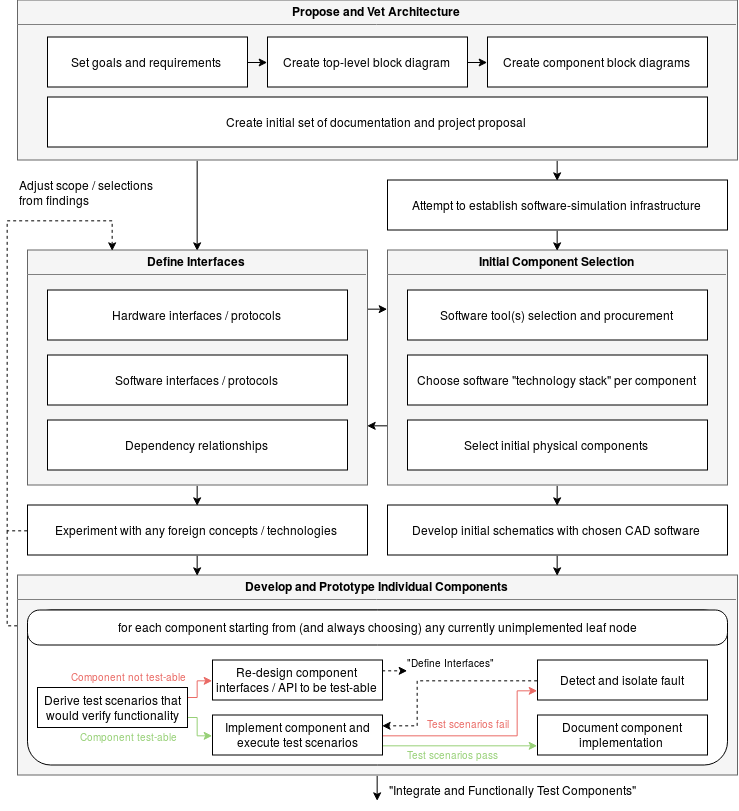
\includegraphics[width=\linewidth]{../src/im/workflow_1}
	\caption{A flexible workflow diagram that attempts to capture our ideal
		process for initial prototype and development work.}
	\label{fig:workflow_1}
\end{figure}

\begin{figure}[H]
	\centering
	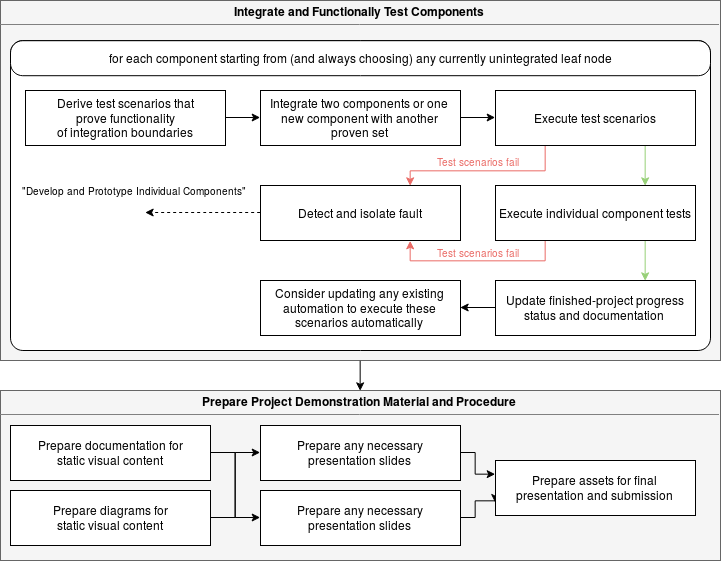
\includegraphics[width=\linewidth]{../src/im/workflow_2}
	\caption{The remaining stages of the workflow diagram that captures our
		intended process for bringing the project to completion.}
	\label{fig:workflow_2}
\end{figure}

\end{document}
